\documentclass[11pt]{article}
\title{Symmetry 9}
\author{https://github.com/heptagons/lenses}
\date{2024/1/12}

\usepackage{graphicx}

\usepackage[margin=0.75in]{geometry}
\usepackage{float} % {figure}{H}
\usepackage{amsmath} % \dfrac

\begin{document}

\maketitle
\begin{abstract}
Symmetry 9
\end{abstract}

\section{Stars and lenses}

\begin{figure}[h]
\centering
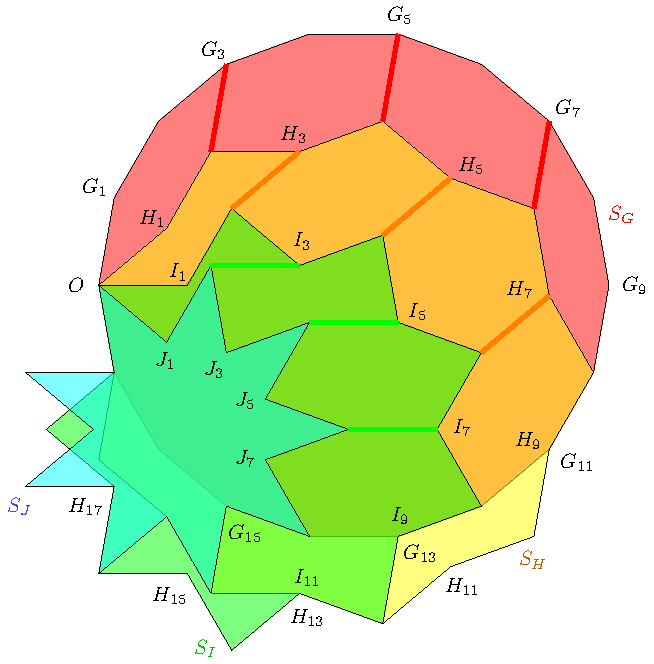
\includegraphics[scale=1]{stars-9}
\caption{Symmetry $9$ stars $\{S_G,S_H,S_I,S_J\}$ dissected with vectors to get symmetry-9 hexagonal lenses.}
\label{fig:stars-9}
\end{figure}

Figure \ref{fig:stars-9} show the disposition of the symmetry $9$ four stars $\{S_G,S_H,S_I,S_J\}$. We denote the $18$ vertices of every star as $\{0,X_1,...,X_{17}\}$ where $X = \{G,H,I,J\}$. Only some vertices are labeled in the figure

\section{Rhombus}

\section{Lenses}

\section{Crowns}


\end{document}

